\documentclass[11pt, oneside]{article}   	% use "amsart" instead of "article" for AMSLaTeX format
\usepackage[margin=0.5in]{geometry}                		% See geometry.pdf to learn the layout options. There are lots.
\usepackage[numbers]{natbib}
\usepackage{wrapfig}
\usepackage[autostyle,english=american]{csquotes} % because I hate the `` '' latex quote style and also i am lazy 
\MakeOuterQuote{"}
\geometry{letterpaper}                   		% ... or a4paper or a5paper or ... 

%\geometry{landscape}                		% Activate for for rotated page geometry
%\usepackage[parfill]{parskip}    		% Activate to begin paragraphs with an empty line rather than an indent
\usepackage{graphicx}				% Use pdf, png, jpg, or eps§ with pdflatex; use eps in DVI mode
								% TeX will automatically convert eps --> pdf in pdflatex		
\usepackage{amssymb}
\newcommand{\rhts}{\textsc{RosettaHTS}\ } 
\title{Progress Report}
\author{Sam DeLuca}
%\date{}							% Activate to display a given date or no date

\begin{document}
\maketitle
\section{Aim I: Develop protein-ligand docking guided by QSAR-derived pharmacorphore maps}
Optimization of the \rhts docking algorithm has continued, with the current version capable of frequently obtaining a \textless 2.0 \AA\ pose within 25 models during a self docking study.
The current protocol initially uses coarse grained docking with a grid based encoding shape complimentarily and hydrogen bonding information.  
Based on the initial prediction, fine grained docking using the Rosetta energy function is performed.  
During fine grained docking, the backbone, side chains, and ligand are flexible. 
The current docking protocol can process a single ligand in 15-30 minutes, depending on the size of the protein.

\subsection{The Rosetta energy function has a limited ability to perform rank order prediction.}
The current implementation of the Rosetta energy function is limited in its ability to accurately predict binding affinity.
While correct poses of a single ligand can frequently be distinguished using binding energy\citep{Davis:2009fx}, comparison of the energies of different ligands is generally poor\citep{Kaufmann:2009cq}.

Optimization studies the \rhts algorithm suggest that in many cases, normalization can be effective in improving the quality of rank order prediction for specific protein targets.  
However the optimal parameters of the normalization method were found to be substantially different for each protein target.  
Given this, it is unlikely that a optimal scoring function will be obtained using a linear combination of weighted scoring terms. 

\subsection{Integration of Chemical Information with \rhts}
To address the problem described above, a machine learning approach was undertaken that allows the ligand binding pose to be directly combined with chemical information.
A set of fingerprint descriptors describing the protein-ligand interface and protein binding site were developed based on Radial Distribution Functions (RDFs).  
The RDF represents the probability distribution of atoms existing at varying distances from each other with the protein ligand interface and protein binding site.  
Importantly, RDFs can be "colored" with scoring information, allowing for the creation of fast fingerprint descriptors representing the 3D geometry of the protein ligand binding site, and the distribution of chemical properties within that binding site.  
The RDFs take the form of $g(r) =\frac{1}{2}\sum\limits_{i,j}score_{ij}e^{-B(r-r_{ij})^2}$ Where $r$ is a radius bin, $r_{ij}$ is the distance between two atoms, $score_{ij}$ is the interaction score for those two atoms, and $B$ is a smoothing factor.  
The Rosetta RDF fingerprints are computed using 100 bins, with the radius of each bin incremented by 0.1 \AA.  

The RDFs computed by Rosetta represent only the protein interface and protein pocket, but do not directly encode information about the ligand itself.  
To accomplish this, a set of cheminformatics descriptors\citep{Mueller:2012gn} were computed. 
These descriptors are a combination of scalar, 2D and 3D descriptors representing a range of chemical and geometric properties of the ligand. 
The complete set of 6800 descriptor columns is used as the input of a neural network which is trained to predict $-log(K_{i})$. 

While neural networks are frequently used to predict small molecule activity\citep{Hecht:2008gs, Mueller:2012gn, Gohlke:2002in}, these networks are typically trained to predict activity with respect to a single drug target or narrow class of targets.  
By integrating information about the protein binding site and protein-ligand interface, we hope to be able to train the network to recognize general patterns associated with binding activity.  
The ability to recognize these general patterns would result in a single model with predictive power over a wide range of protein targets and ligand chemical space.  
This would improve the quality of perform vHTS screens and QSAR studies on targets for which protein structures exist, but few active and inactive compounds are known. 
\begin{wrapfigure}{r}{0.5\textwidth}
   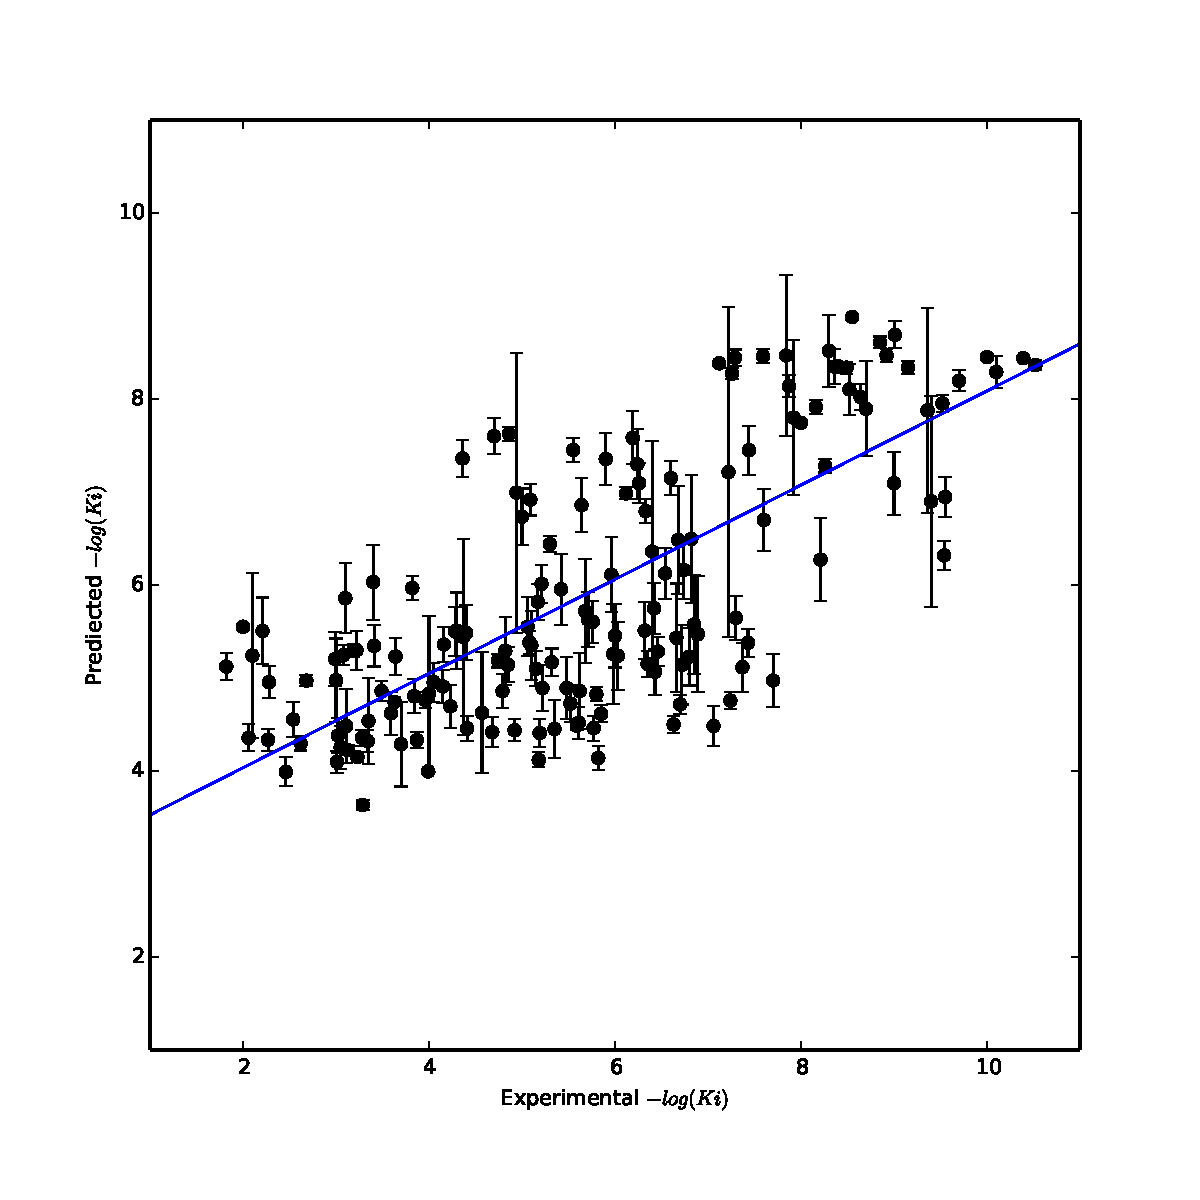
\includegraphics[width=0.48\textwidth]{figures/crossval_correlation.pdf} % requires the graphicx package
   \caption{Correlation between predicted and experimetnal $-log(K_{i})$ based on the independent partition of the training cross-validation, with linear regression model plotted in blue. }
   \label{fig:crossval}
\end{wrapfigure}

A neural network was trained using a set of 209 protein-ligand pairs from the Community Structure Activity Resource (CSAR)\citep{Smith:2011gb}.  
The ligands in this training set have experimentally determined $-log(K_{i})$ between 2 and 11.  
Each ligand was docked into the protein 100 times, and the top 10 binding poses by Rosetta interface energy were selected for training. 
The initial neural network was trained using the full set of 6800 descriptors using a 72 fold cross validation with separate independent and monitoring partitions.  
Ligand poses from the independent partitions exhibited an $R^{2}$ correlation of 0.50 between the predicted and experimental $-log(K_{i})$ (Figure \ref{fig:crossval}).

While this correlation is not unreasonable, the possibility exists that the model is of limited general applicability.  
To determine if the model is capable of making predictions outside the 209 systems in the training set, an additional 33 systems were selected from the Pdbbind database.  
These systems were docked 100 times, and the top scoring pose by Rosetta binding energy was scored using the neural network.
The resulting predicted $-log(K_{i})$ was plotted against the actual Ki.
The resulting correlation had an $R^{2}$ of 0.47, similar to that of the independent cross validation partition, indicating that the network has some ability to generalize.
Furthermore, the correlation produced by the ANN predictions is improved over the correlation between Rosetta $\Delta\Delta G$ energy and experimental $-log(K_{i})$, with an $R^{2}$ of 0.17. (Figure \ref{fig:indepval})
\begin{figure}[htbp]
   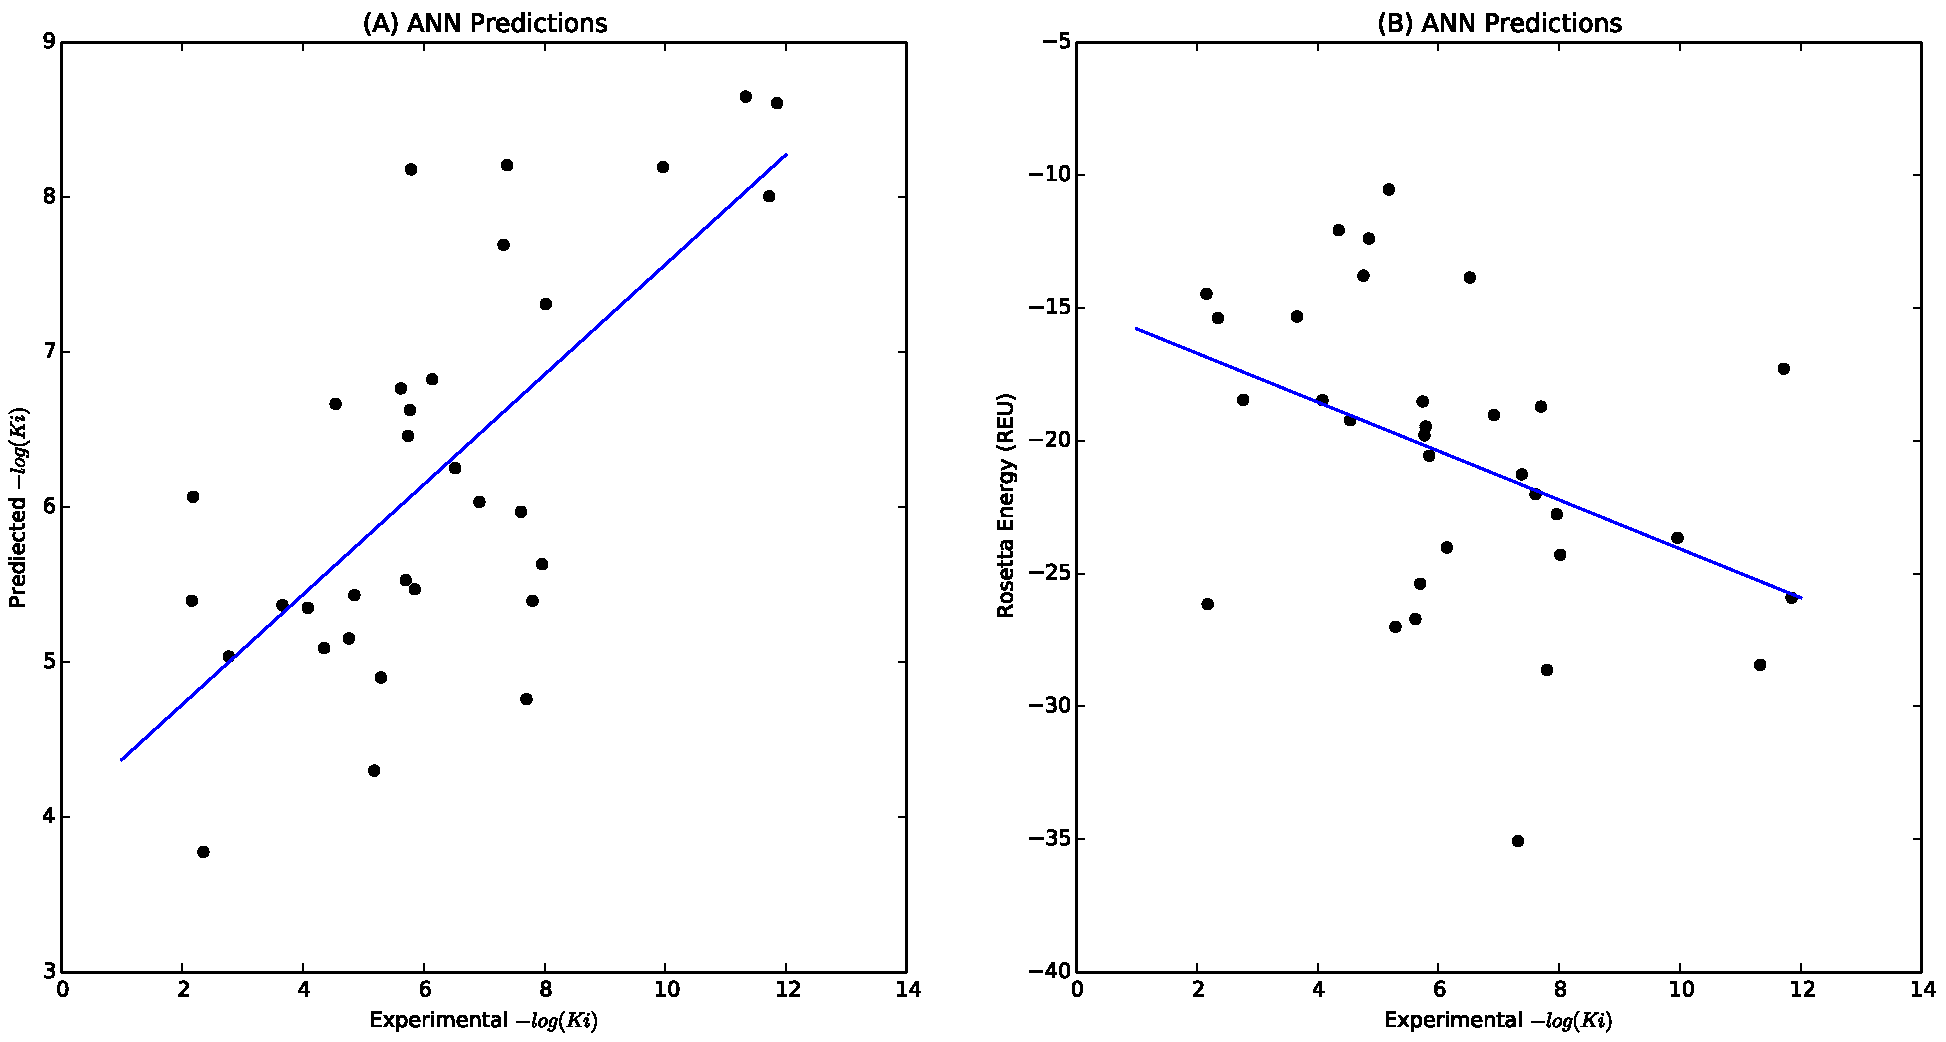
\includegraphics[width=1.0\textwidth]{figures/independent_correlation.pdf} % requires the graphicx package
   \caption{Correlation of predicted $-log(K_{i})$ (A), and Rosetta energy (B) with experimental $-log(K_{i})$  based on the PDBBind derived benchmarking set. Linear regression model plotted in blue.}
   \label{fig:indepval}
\end{figure}

As the goal of \rhts is to distinguish between active and inactive ligands, ROC curves are also a useful metric for assessing the performance of the model.
ROC curves were generated using the method described by Fan et al. \citep{Fan:2009kh}
The ROC curve analysis indicates that at least for the small 33 system independent set, \rhts is effectively able to distinguish nanomolar binders from weaker binding compounds.

The current neural network was trained on only a small subset of chemical and protein space, and includes only compounds with measurable binding affinities.  
While the network does exhibit some ability to predict binding affinity across a range of targets, its ability is likely limited. 
To assess the extent of these limitations, two large screening benchmark sets, Directory of Useful Decoys - Enhanced(DUD-E)\citep{Mysinger:2012hu} and DEKOIS 2.0\citep{Bauer:2013de} are being prepared for screening using \rhts.
These libraries consist of a large set of known inhibitors for a wide range of protein targets, and a set of predicted inactive "decoys".  
In both cases, the decoys are derived through property matching of a range of chemical property descriptors, and structure based filtering to remove structural analogs of known actives.   
The advantage of this approach is that a large set of inactive compounds can easily be assembled.
The disadvantage of decoy prediction approach is that active compounds can be inadvertently included in the dataset, skewing the measured performance of the metric.
By testing \rhts using multiple benchmark sets compiled using different decoy generation methods, it will be more possible to determine if performance is being majorly impacted by pathologies in the decoy generation process. 

\subsection{Future Directions}
To improve the quality of the neural network, the size of the training dataset is being increased.  
In addition to the 209 compounds from the CSAR dataset,  approximately 8500 compounds were selected from ChEMBL\citep{Gaulton:vaa}.
Compounds were selected to have known $-log(K_{i})$ values when docked into targets with crystal structures of \textless 2.0 \AA resolution and high quality binding sites that did not contain cofactors.
Additionally, compounds were filtered to have atoms with assignable Rosetta atomtypes, assignable BCL atomtypes, and molecular weight of 150-500.
While the compounds selected with known $-log(K_{i})$ values had a relatively wide range of binding affinity, it will be useful to have a set of compounds which are experimentally confirmed to be inactive.
A set of 1800 additional compounds were selected from ChEMBL which were reported to have 0\% activity vs targets in the CSAR and ChEMBL active datasets.
As these compounds were verified to have no binding activity, but typically do not have measured $-log(K_{i})$ values, the $-log(K_{i})$ value was set to 0.0. 
The combined active and inactive compounds from the CSAR and ChEMBL datasets will be used to train and optimize a new neural network which should exhibit more accurate predictions across a wider range of chemical and protein conformational space. 


\subsection{Publication and Defense Plan}
Following the completion of the benchmarking work described above, a paper describing the \rhts method will be published.
This paper will describe the implementation of \rhts as well as the results of the DUD-E and DEKOIS benchmarks.
The paper will be targeted for publication in PLoS Computational Biology or Journal of Medicinal Chemistry.

The PhRMA foundation pre-doctoral fellowship which funds my current work expires at the end of the year.  
As a result, I would like to defend my thesis describing \rhts in January. 
Following the defense of my thesis, I will begin a 1 year post-doctoral position in the Meiler lab.
The purpose of this position will be to continue to advance the development and application of Rosetta ligand docking technology.
After this short post-doctoral position, I plan on pursuing an academic postdoc. 

\bibliographystyle{ieeetr}
\bibliography{bibliography}

\end{document}  